% ============================================================
% Final Project Report (Draft) — Spot To Go
% Prepared for supervisor review and feedback
% ============================================================

\documentclass[12pt, a4paper]{article}

% --- Packages ---
\usepackage[margin=2.5cm]{geometry}
\usepackage{setspace}
\usepackage{titlesec}
\usepackage{parskip}
\usepackage{booktabs}
\usepackage{array}
\usepackage{natbib}
\usepackage{times}
\usepackage{graphicx}
\usepackage{float}
\usepackage{tikz}
\usetikzlibrary{arrows.meta, shapes.geometric, positioning, calc, fit, shapes.multipart}

% hyperref is loaded last (best practice) so it can patch the other packages
% correctly; loading it too early caused duplicate figure/page PDF anchors.
\usepackage{hyperref}
\usepackage{bookmark}

\doublespacing

% --- Clickable, coloured cross-references and citations ---
\hypersetup{
    colorlinks=true,
    linkcolor=black,
    citecolor=black,
    urlcolor=blue!60!black
}

% --- Section formatting ---
\titleformat{\section}{\large\bfseries}{\thesection.}{0.5em}{}
\titleformat{\subsection}{\normalsize\bfseries}{\thesubsection}{0.5em}{}

% --- Screenshot grid helper ---
\newcommand{\shot}[3]{%
  \begin{minipage}[t]{#1}
    \centering
    \includegraphics[width=\linewidth]{images/#2}\\[2pt]
    {\footnotesize #3}
  \end{minipage}%
}

% ============================================================
\begin{document}

% --- Title Page (manual, so front matter can be numbered i, ii, ... ) ---
\pagenumbering{roman}
\thispagestyle{empty}
\begin{center}
    \vspace*{2cm}

    {\LARGE \textbf{Spot To Go: A Location-Based Android Application}} \\[0.6em]
    {\large \textbf{for Restaurant Discovery with Video Integration}} \\[2.5em]

    {\large Final Project Report} \\[3em]

    {\large August 2026} \\[2em]

    \vfill
\end{center}
\clearpage

% ============================================================
% --- Abstract ---
\begin{abstract}
\noindent
Choosing where to eat is still driven largely by star ratings and short text reviews, neither of which conveys the atmosphere, food presentation, or overall experience of a place particularly well. This report presents \textbf{Spot To Go}, an Android application that pairs a live, location-aware map of nearby restaurants with a direct link to a real short-form video of each one, so that a user can form a more grounded impression before deciding where to go. The application is built in Kotlin using Jetpack Compose and Navigation Compose, draws the user's position from the Fused Location Provider, renders restaurants on the Google Maps SDK, and gates the experience behind live Firebase Authentication. Video previews and turn-by-turn directions are delegated to the platform apps the user already trusts through Android intents. This document restates the project aim and objectives with their current status, revisits and updates the related literature, presents the system design using UML and flowchart notation, describes the implemented screens, and evaluates the work carried out so far. Eleven screens are fully implemented and connected, authentication has been tested end-to-end on a physical device, and the remaining work --- principally replacing the placeholder restaurant data with a live Google Places API integration --- is scoped and scheduled. The report closes with a project schedule and a clear statement of how the work will be taken forward to completion.
\end{abstract}

% ============================================================
% --- Acknowledgements ---
\newpage
\section*{Acknowledgements}
\addcontentsline{toc}{section}{Acknowledgements}

I would like to thank my project supervisor for their continued guidance, and in particular for the detailed feedback on the earlier draft of this report, which directly shaped the structure and the additions presented here. I am grateful for the time taken to review the work and to suggest concrete improvements to its academic presentation.

I would also like to thank my family and friends for their patience and encouragement throughout the project, and the wider Android and open-source developer community, whose freely available documentation and examples made much of the implementation possible.

Finally, I acknowledge the developer tools and platform services --- Android Studio, the Google Maps and Places platforms, and Firebase --- that provided the foundation on which this application was built.

% ============================================================
% --- Front matter listings ---
\newpage
\tableofcontents
\newpage
\listoffigures
\clearpage

% --- Body starts here; restart page numbering at 1 ---
\pagenumbering{arabic}

% ============================================================
\section{Introduction}

\subsection{Overview}

This report documents the design, implementation, and current progress of ``Spot To Go,'' an Android application that allows users to discover nearby restaurants on an interactive map and access real-life video previews before deciding where to go. It follows on from the dissertation proposal submitted earlier in the project and reflects the system as it has actually been built, rather than only as it was originally planned.

\subsection{Background and Context}

The way people decide where to eat has shifted with the devices they carry. A smartphone now sits between the diner and the decision at almost every stage: locating options, comparing them, reading what others thought, and navigating to the chosen place. Location-based services, which tailor information to a device's real-world position, have become the connective tissue of this experience, and mapping and place-search platforms expose that capability to any application through well-documented programming interfaces \citep{google_places, android_location}. At the same time, the format in which people consume and trust information about places has changed. Short-form video --- popularised by platforms such as TikTok, Instagram Reels, and YouTube Shorts --- has grown into one of the most widely consumed types of online content, and a substantial and growing share of daily media time is now spent watching it \citep{datareportal2024, montag2021}. For a decision as experiential as choosing a restaurant, a fifteen-second clip of the room, the plates, and the people in it communicates something that a numerical average cannot.

\subsection{Problem Statement}

The core problem motivating this project is the gap between how restaurants are \emph{presented} on discovery platforms and how diners actually \emph{form impressions} of them. Existing platforms present restaurants primarily through star ratings and short text reviews. Both compress a rich, multi-sensory experience into a single number or a few sentences, and both struggle to communicate atmosphere, portion size, food presentation, and the general feel of a place. Star ratings in particular aggregate away exactly the detail a diner is trying to judge, and text reviews are slow to read and easy to distrust \citep{dellarocas2003, cheung2009}. Short-form video, by contrast, has become one of the most credible and effective formats for conveying real-world experience, because it shows the place rather than describing it \citep{kaplan2010, montag2021}. Yet mainstream restaurant-discovery tools do not place that video directly alongside the map and the ``go here now'' decision; a user must typically leave the map, open a separate video app, and search by hand. Spot To Go addresses this gap by pairing a live map of nearby restaurants with a direct, one-tap link to a real video of each one, so that a user can make a more informed decision before travelling anywhere.

\subsection{Aim and Contributions}

The aim of the project, stated in full in Section~2, is to design and build an Android application that unifies location-aware restaurant discovery and short-form video preview in a single, coherent flow. In meeting that aim, the work presented here makes three practical contributions. First, it delivers a complete, working Android application of eleven connected screens, built with a current, industry-standard toolset (Kotlin and Jetpack Compose) rather than a legacy one. Second, it demonstrates a clean separation between the user interface and its data sources, designed specifically so that the placeholder restaurant data can be replaced with a live Google Places API integration without reworking any screen. Third, it grounds the design in an updated review of the relevant literature and expresses that design through standard UML and flowchart notation, so that the system can be understood and extended by others.

\subsection{Report Structure}

This document is structured to give an honest account of progress: it restates the aim and objectives with their current status (Section~2), revisits and updates the literature review (Section~3), describes the system as designed using UML and flowchart notation (Section~4) and as implemented (Section~5), evaluates what has been tested so far (Section~6), updates the risk and ethical analysis in light of the real authentication system now in place (Section~7), and closes with a project schedule and a clear statement of what remains to be built (Sections~8 and~9). Since the purpose of this draft is to gather feedback before the final phase of work, sections that describe incomplete features are marked explicitly rather than glossed over.

% ============================================================
\section{Aim and Objectives}

\subsection*{Aim}

The aim of the project is unchanged from the proposal: to design and develop an Android application that enables users to discover nearby restaurants through an interactive, location-aware map interface, and to access associated video content that supports informed decision-making.

\subsection*{Objectives and Current Status}

The table below restates the seven objectives defined in the proposal and reports their current status, based on the implementation described in Sections 4 and 5.

\begin{center}
\renewcommand{\arraystretch}{1.3}
\begin{tabular}{p{0.07\textwidth} p{0.63\textwidth} p{0.22\textwidth}}
\toprule
\textbf{No.} & \textbf{Objective} & \textbf{Status} \\
\midrule
1 & Integrate the Google Maps SDK to render an interactive map centred on the user's real-time GPS location. & Achieved \\
2 & Implement location-based restaurant discovery using the Google Places API. & Not yet started \\
3 & Develop a restaurant detail screen presenting name, rating, distance, and description. & Achieved \\
4 & Integrate video content from YouTube or TikTok per restaurant. & Achieved \\
5 & Implement a navigation feature that launches Google Maps directions to a selected restaurant. & Achieved \\
6 & Design a keyword-based search interface to filter nearby restaurant results. & Partially achieved \\
7 & Evaluate the application through functional testing against each objective. & In progress \\
\bottomrule
\end{tabular}
\end{center}

Objective 1 is complete: the map centres on the device's real GPS position using the Fused Location Provider. Objectives 3, 4, and 5 are complete and have been exercised on a physical device. Objective 6 is partially achieved — a working search bar filters the restaurants currently loaded into the app, but it filters an in-memory list rather than passing the keyword to a live Places API query, since Objective 2 has not started yet. Objective 2 is the immediate next piece of work, discussed further in Section 8. Objective 7 is ongoing: functional checks have been carried out informally on a physical device during development, but the structured, objective-by-objective test documentation proposed in Section 5.7 of the original proposal has not yet been written up formally.

% ============================================================
\section{Critical Review of Related Literature}

The development of Spot To Go continues to be informed by four interconnected areas of research: location-based services, restaurant recommendation systems, the role of video-based user-generated content in consumer decision-making, and Android application development. This section restates and, where relevant, updates the literature review from the proposal in light of the implementation decisions made since.

\subsection{Location-Based Services}

Location-based services (LBS) use the geographic position of a device to deliver contextually relevant information or functionality. \citet{schiller2004} describe how GPS positioning, mobile networks, and application logic combine to enable this class of context-sensitive application. \citet{dey2001} extends this through context-aware computing — systems that adapt to the user's physical environment automatically rather than through manual configuration. This principle is realised directly in the implemented app: the Fused Location Provider reads the user's position automatically on the Map and Directions screens, with no manual location entry required anywhere in the interface.

\citet{bao2012} shows that combining location data with user preference modelling improves the relevance of place-based recommendations. As in the proposal, this project does not implement preference modelling; the current architecture, in which the map consumes restaurant data through a single repository interface, is designed so that such a model could be introduced later without changing the screens that depend on it.

\subsection{Restaurant Recommendation Systems}

\citet{adomavicius2005} identify content-based filtering, collaborative filtering, and hybrid approaches as the dominant paradigms for recommender systems. The proposal committed to a simplified content-based approach: keyword-based search against the Google Places API. At the time of writing, this specific integration has not yet been built — the search bar currently filters a small, hardcoded set of restaurants used as placeholder data during development of the surrounding screens. This distinction matters for how the literature review should be read: the architectural decision to filter by keyword is already implemented and working, and the remaining task is to point that same mechanism at live Places API data instead of the placeholder list. Once complete, the Places API's built-in ratings and review counts will still provide the aggregated collaborative signal described in the proposal, without the application needing to implement that logic independently.

\subsection{Video-Based User-Generated Content and Consumer Decisions}

\citet{dellarocas2003} frames user-generated content as a digital extension of word-of-mouth communication with a measurable influence on purchasing decisions. \citet{kaplan2010} and \citet{cheung2009} both identify video specifically as more credible and more effective than text at communicating atmosphere and experiential quality. More recent work confirms that this shift has accelerated with the rise of short-form video: \citet{montag2021} examine why platforms such as TikTok hold attention so effectively, linking their appeal to the immediacy and authenticity of short, real-world clips, while \citet{barta2023} show empirically that short-form video content on TikTok measurably shapes consumer attitudes and intentions, particularly when the content feels genuine rather than staged. The scale of this behaviour is now considerable: industry measurement reports place short-form video among the most consumed categories of online content, accounting for a large and rising share of daily media time \citep{datareportal2024}. These newer sources strengthen, rather than replace, the older foundational work: the mechanism Dellarocas described in 2003 is the same one now operating at far greater scale through video. This is the central premise the app demonstrates in working form: from the restaurant detail screen, a user can open a real video of the restaurant with a single tap, and the app also offers a second path to a TikTok search for the same restaurant. Both actions hand off to the platform the user already trusts, rather than attempting to recreate video playback inside the app.

\subsection{Android Mobile Application Development}

\citet{wasserman2010} identifies device fragmentation, limited processing resources, and state management across screen transitions as recurring challenges in mobile development. While that analysis remains a useful framing of the problem space, the tooling has moved on considerably since it was written. The proposal addressed state management through the Activity lifecycle; the implemented app instead adopts Jetpack Compose and Navigation Compose, now Google's officially recommended toolkit for building native Android user interfaces \citep{jetpack_compose}, in which each screen is a composable function managed by a single navigation host. This is a deviation from the proposal, and Section 4.1 explains the reasoning behind it in full. In short, the underlying challenge Wasserman describes --- predictable state across navigation events --- is still the driving design concern; only the specific mechanism used to solve it has changed, in line with current Android development practice.

The Google Play Services suite — the Maps SDK, the Fused Location Provider, and (prospectively) the Places API — remains the standardised, well-documented toolset underpinning the location-aware features of the app, exactly as anticipated in the proposal.

% ============================================================
\section{System Design}

\subsection{Application Architecture}

The proposal specified a Java, single-Activity-per-screen architecture. The implemented application instead uses Kotlin with Jetpack Compose, in which every screen is a composable function rendered within one Activity (\texttt{MainActivity}) and connected through a single Navigation Compose host. This is a deliberate deviation from the original plan, made for three reasons. First, Kotlin is explicitly accepted as an alternative to Java in the project brief, so the change introduces no scope risk. Second, Compose is Google's current recommended toolkit for new Android UI work, and using it demonstrates familiarity with present-day Android practice rather than a superseded one. Third, and most practically, Compose's state-driven model turned out to simplify exactly the problem the proposal was most concerned about: passing the selected restaurant between the map, detail, video, and directions screens is handled by a single piece of shared state read by each screen, rather than by packaging data into each Activity's launch \texttt{Intent} by hand.

Figure~\ref{fig:prototype} shows the original hand-drawn prototype that the screen set was designed against. Eleven screens have been implemented in total: a Splash screen, Login and Registration, a Home screen, the Map, Restaurant Detail, a Video screen, a TikTok link screen, Directions, Contact Us, and a Privacy Policy screen. The last four of these — the TikTok link screen, Contact Us, and Privacy Policy — extend beyond the six views sketched in the original prototype; they were added to give the video feature a second, working path (TikTok as well as YouTube) and to meet ordinary expectations of a publishable app (a contact channel and a privacy statement), without changing the core flow the prototype describes.

\begin{figure}[H]
    \centering
    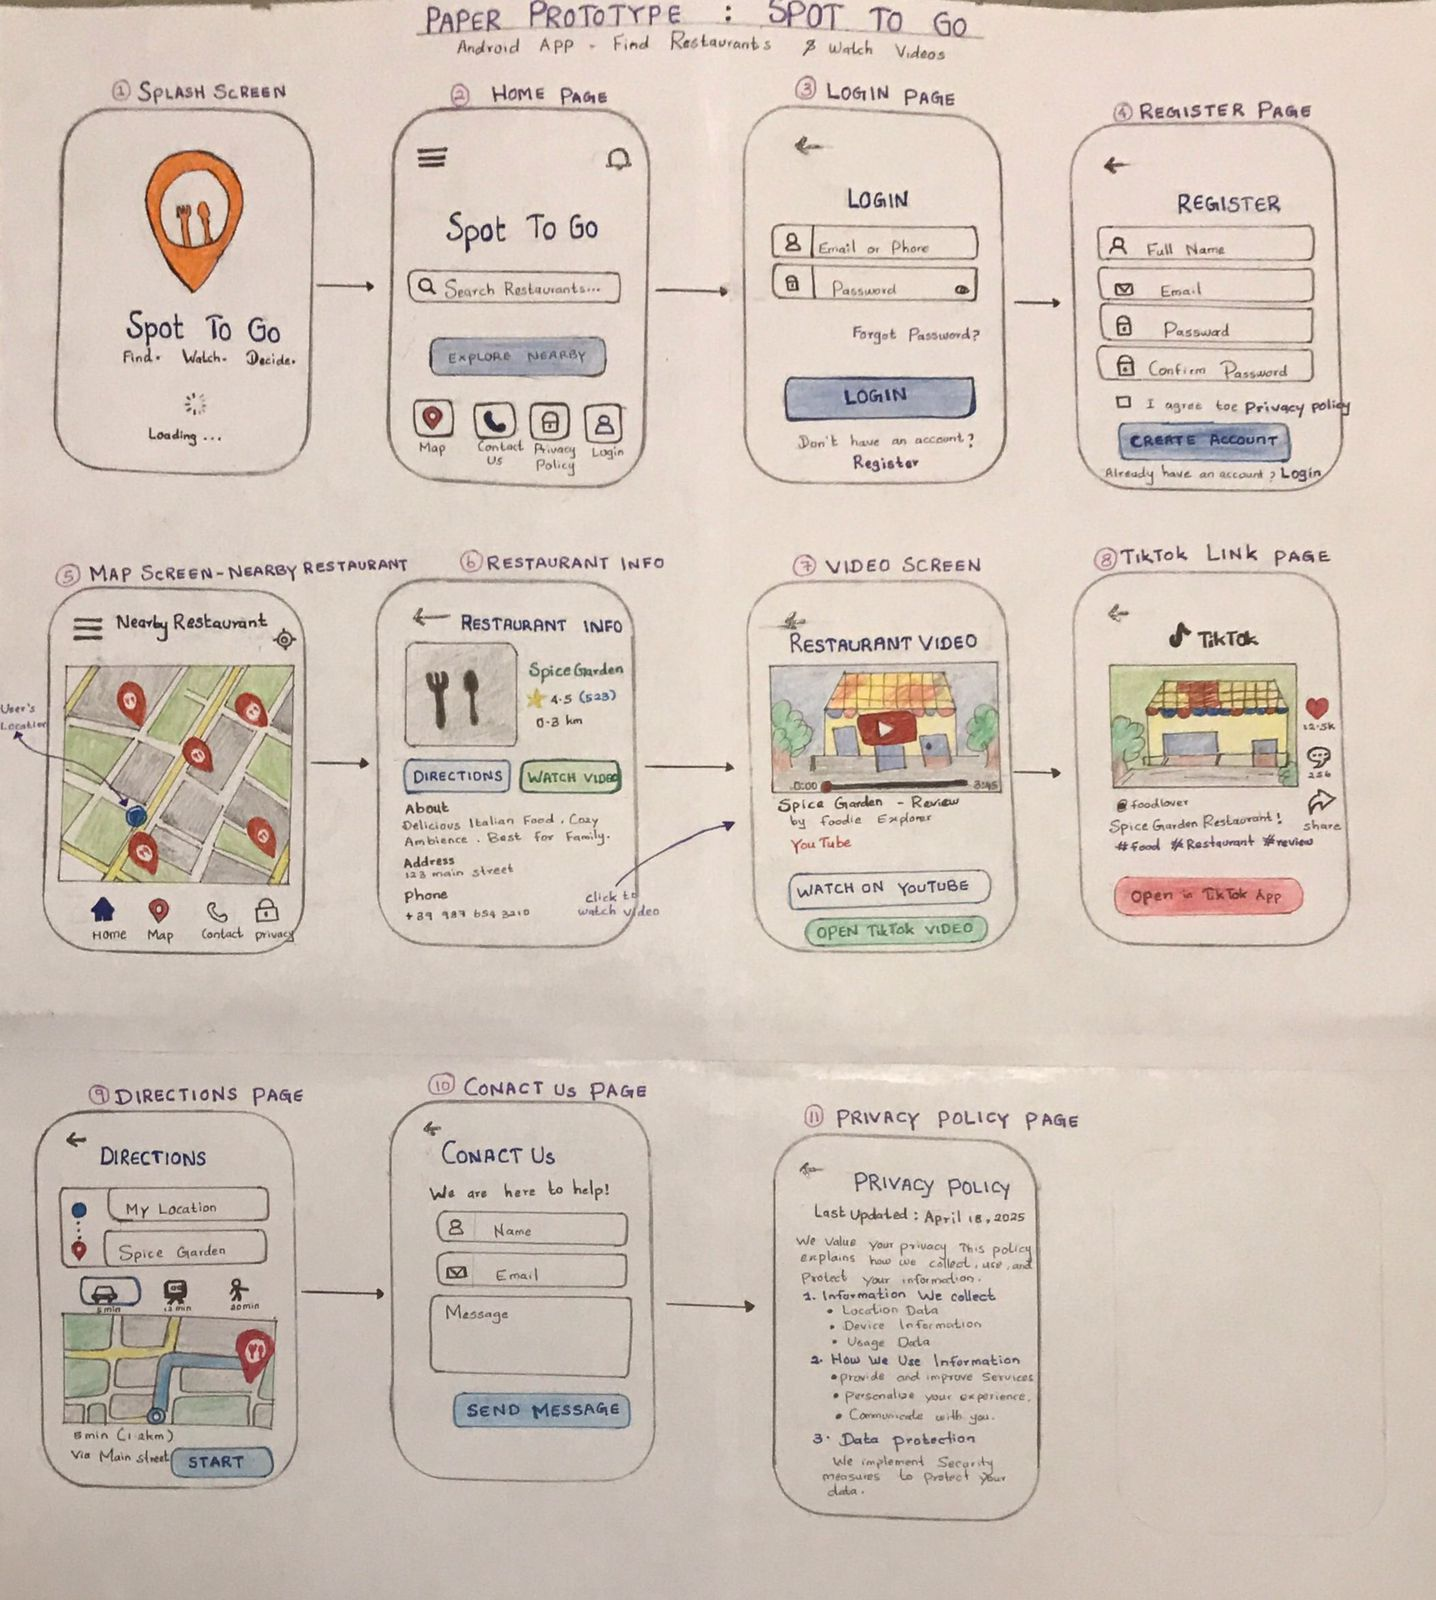
\includegraphics[width=0.92\textwidth]{images/prototype.jpeg}
    \caption[Original hand-drawn prototype of the application.]{Original hand-drawn prototype of the Spot To Go application, showing the planned flow across login, home search, the map with restaurant markers, restaurant detail, video playback, and directions. This layout directly informed the screen set described above.}
    \label{fig:prototype}
\end{figure}

Figure~\ref{fig:navmap} traces the same eleven screens as an explicit navigation map, showing every transition a user can actually make, including the two secondary screens (Contact Us and Privacy Policy) and the bottom navigation bar added during testing (Section 6.1) that lets a user return from the Map screen to Home.

\begin{figure}[H]
\centering
\resizebox{\textwidth}{!}{%
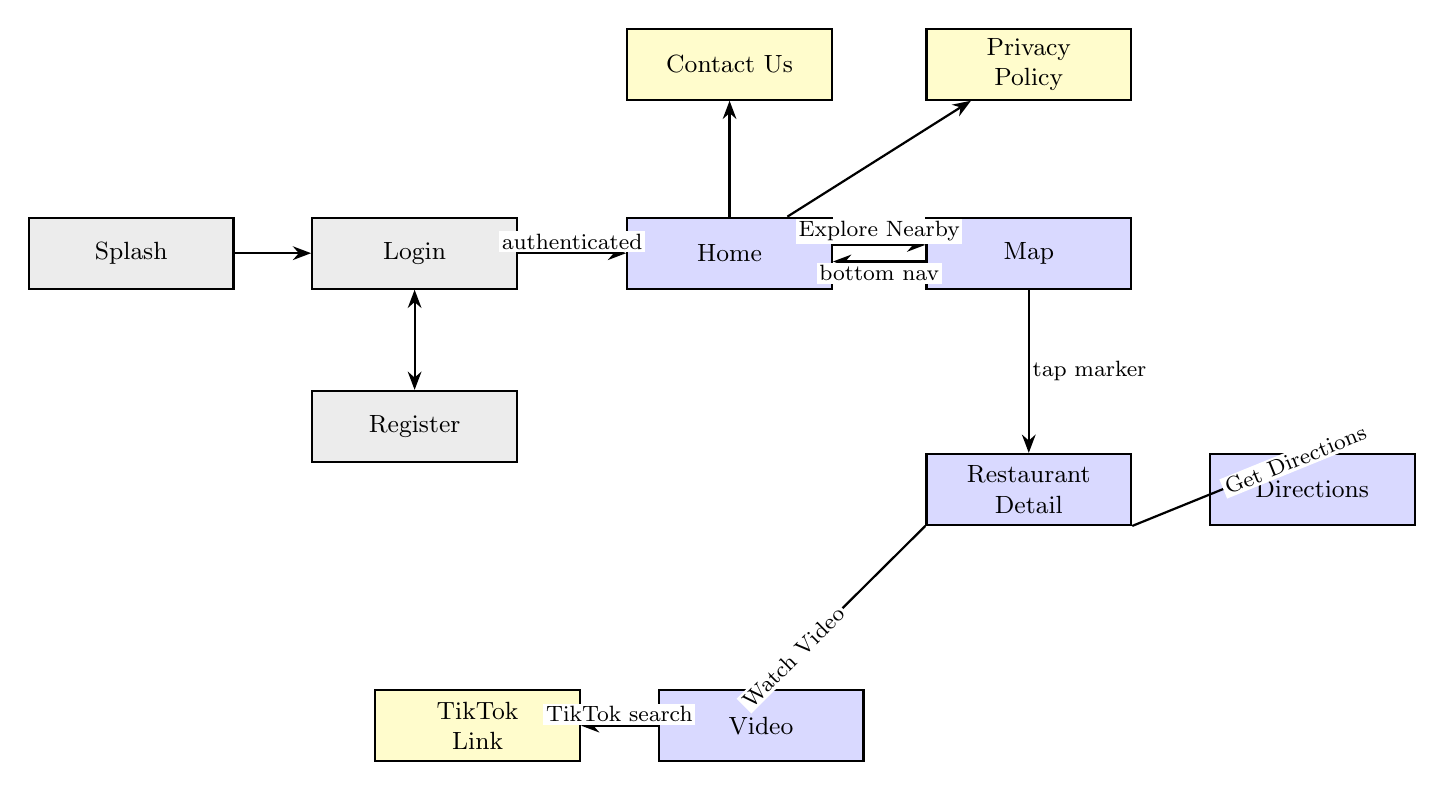
\begin{tikzpicture}[
    core/.style={
        rectangle, draw, thick, fill=blue!15,
        minimum width=2.6cm, minimum height=0.9cm,
        align=center, font=\small
    },
    auth/.style={
        rectangle, draw, thick, fill=gray!15,
        minimum width=2.6cm, minimum height=0.9cm,
        align=center, font=\small
    },
    aux/.style={
        rectangle, draw, thick, fill=yellow!20,
        minimum width=2.6cm, minimum height=0.9cm,
        align=center, font=\small
    },
    >=Stealth, thick,
    lbl/.style={font=\footnotesize, fill=white, inner sep=1pt}
]

\node[auth] (splash)   at (0,    0)   {Splash};
\node[auth] (login)    at (3.6,  0)   {Login};
\node[auth] (register) at (3.6, -2.2) {Register};
\node[core] (home)     at (7.6,  0)   {Home};
\node[aux]  (contact)  at (7.6,  2.4) {Contact Us};
\node[aux]  (privacy)  at (11.4, 2.4) {Privacy\\Policy};
\node[core] (map)      at (11.4, 0)   {Map};
\node[core] (detail)   at (11.4, -3)  {Restaurant\\Detail};
\node[core] (video)    at (8,   -6)   {Video};
\node[aux]  (tiktok)   at (4.4, -6)   {TikTok\\Link};
\node[core] (dir)      at (15,  -3)   {Directions};

\draw[->] (splash) -- (login);
\draw[<->] (login) -- (register);
\draw[->] (login) -- node[lbl, above]{authenticated} (home);
\draw[->] (home) -- (contact);
\draw[->] (home) -- (privacy);
\draw[->] ([yshift= 3pt]home.east) -- node[lbl, above]{Explore Nearby} ([yshift= 3pt]map.west);
\draw[->] ([yshift=-3pt]map.west)  -- node[lbl, below]{bottom nav} ([yshift=-3pt]home.east);
\draw[->] (map) -- node[lbl, right]{tap marker} (detail);
\draw[->] (detail.south west) -- node[lbl, left, sloped]{Watch Video} (video.north);
\draw[->] (detail.south east) -- node[lbl, right, sloped]{Get Directions} (dir.north);
\draw[->] (video) -- node[lbl, above]{TikTok search} (tiktok);

\end{tikzpicture}%
}
\caption[Screen navigation map for Spot To Go.]{Screen navigation map for Spot To Go. Gray nodes are the authentication screens, blue nodes are the core discovery flow, and yellow nodes are secondary screens reached from Home. The Map-to-Home bottom navigation link was added in response to a usability issue found during testing (Section 6.1).}
\label{fig:navmap}
\end{figure}

\subsection{Use Case Model (UML)}

Before describing how the system is built, it is worth stating precisely what it lets a user do. Figure~\ref{fig:usecase} presents this as a UML use case diagram. The single human actor, the \emph{User}, interacts with seven use cases enclosed by the system boundary, while three external services --- Firebase, the Google Maps platform, and YouTube/TikTok --- act as secondary actors that the system depends on to fulfil those cases. The diagram also captures two structural relationships that matter for the design: viewing restaurant details \emph{includes} first viewing the map (a user cannot open a detail screen without selecting a marker), and both watching a video and getting directions \emph{extend} the detail use case, since they are optional actions launched from it rather than steps every user must take.

\begin{figure}[H]
\centering
\resizebox{0.92\textwidth}{!}{%
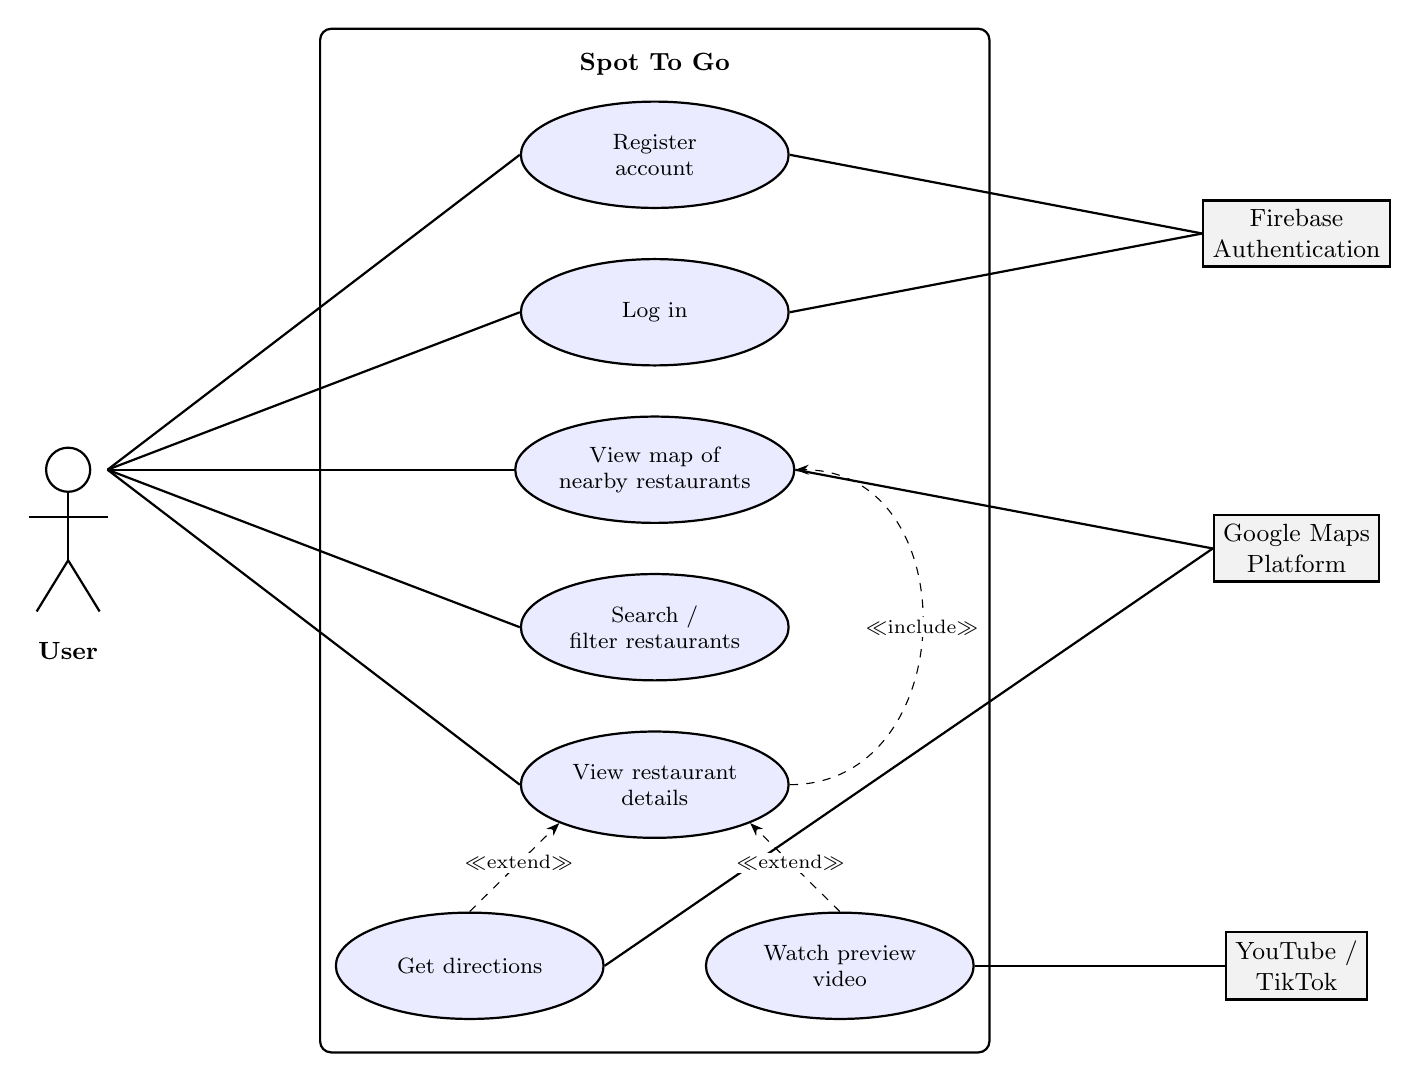
\begin{tikzpicture}[
    actor/.style={font=\small, align=center},
    usecase/.style={
        draw, thick, ellipse, fill=blue!8,
        minimum width=3.4cm, minimum height=1.35cm,
        align=center, font=\footnotesize, inner sep=1pt
    },
    ext/.style={font=\small, align=center},
    >=Stealth
]

% System boundary
\draw[thick, rounded corners] (-1.2,-11.4) rectangle (7.3,1.6);
\node[font=\small\bfseries] at (3.05,1.15) {Spot To Go};

% Use cases (generous vertical spacing so ellipses never touch)
\node[usecase] (register) at (3.05,  0.0)  {Register\\account};
\node[usecase] (login)    at (3.05, -2.0)  {Log in};
\node[usecase] (map)      at (3.05, -4.0)  {View map of\\nearby restaurants};
\node[usecase] (search)   at (3.05, -6.0)  {Search /\\filter restaurants};
\node[usecase] (detail)   at (3.05, -8.0)  {View restaurant\\details};
\node[usecase] (video)    at (5.4,  -10.3) {Watch preview\\video};
\node[usecase] (dir)      at (0.7,  -10.3) {Get directions};

% Primary actor (User) - simple stick figure
\begin{scope}[shift={(-4.4,-4.0)}]
    \draw[thick] (0,0) circle (0.28);
    \draw[thick] (0,-0.28) -- (0,-1.15);
    \draw[thick] (-0.5,-0.6) -- (0.5,-0.6);
    \draw[thick] (0,-1.15) -- (-0.4,-1.8);
    \draw[thick] (0,-1.15) -- (0.4,-1.8);
\end{scope}
\node[actor] at (-4.4,-6.3) {\textbf{User}};

% Secondary actors (external systems)
\node[ext, draw, thick, fill=gray!10, minimum height=0.8cm] (firebase) at (11.2,-1.0) {Firebase\\Authentication};
\node[ext, draw, thick, fill=gray!10, minimum height=0.8cm] (gmaps)    at (11.2,-5.0) {Google Maps\\Platform};
\node[ext, draw, thick, fill=gray!10, minimum height=0.8cm] (yt)       at (11.2,-10.3) {YouTube /\\TikTok};

% User associations
\draw[thick] (-3.9,-4.0) -- (register.west);
\draw[thick] (-3.9,-4.0) -- (login.west);
\draw[thick] (-3.9,-4.0) -- (map.west);
\draw[thick] (-3.9,-4.0) -- (search.west);
\draw[thick] (-3.9,-4.0) -- (detail.west);

% Secondary actor associations
\draw[thick] (register.east) -- (firebase.west);
\draw[thick] (login.east) -- (firebase.west);
\draw[thick] (map.east) -- (gmaps.west);
\draw[thick] (dir.east) -- (gmaps.west);
\draw[thick] (video.east) -- (yt.west);

% include relationship: detail includes map, routed to the RIGHT to avoid crossing other ellipses
\draw[->, dashed] (detail.east) to[out=0, in=0, looseness=1.4]
      node[font=\scriptsize, fill=white, inner sep=1pt, pos=0.5]{$\ll$include$\gg$} (map.east);
% extend relationships: video and directions extend the detail use case
\draw[->, dashed] (video.north) -- node[font=\scriptsize, fill=white, inner sep=1pt, pos=0.55]{$\ll$extend$\gg$} (detail.south east);
\draw[->, dashed] (dir.north) -- node[font=\scriptsize, fill=white, inner sep=1pt, pos=0.55]{$\ll$extend$\gg$} (detail.south west);

\end{tikzpicture}%
}
\caption[UML use case diagram for Spot To Go.]{UML use case diagram for Spot To Go. The User is the single primary actor; Firebase, the Google Maps platform, and YouTube/TikTok are secondary actors the system relies on. Viewing details \emph{includes} viewing the map, and watching a video or getting directions \emph{extend} the detail use case as optional follow-on actions.}
\label{fig:usecase}
\end{figure}

\subsection{Class Design (UML)}

Figure~\ref{fig:classdiagram} expresses the same system as a UML class diagram, focused on the classes that carry behaviour rather than on every composable screen. \texttt{MainActivity} hosts the navigation graph and owns the single shared \texttt{selectedRestaurant} state that the detail, video, and directions screens read. The two repositories, \texttt{AuthRepository} and \texttt{RestaurantRepository}, are the only classes that talk to external services, and \texttt{RestaurantRepository} produces \texttt{Restaurant} objects --- the plain data class that every discovery screen ultimately consumes. Drawing the design this way makes the central architectural decision visible as a structural fact: the screens depend on \texttt{RestaurantRepository}'s interface and on the \texttt{Restaurant} type, not on where the data originates, which is exactly why the planned swap to a live Places-backed repository (Section~8) leaves the screens untouched.

\begin{figure}[H]
\centering
\resizebox{0.96\textwidth}{!}{%
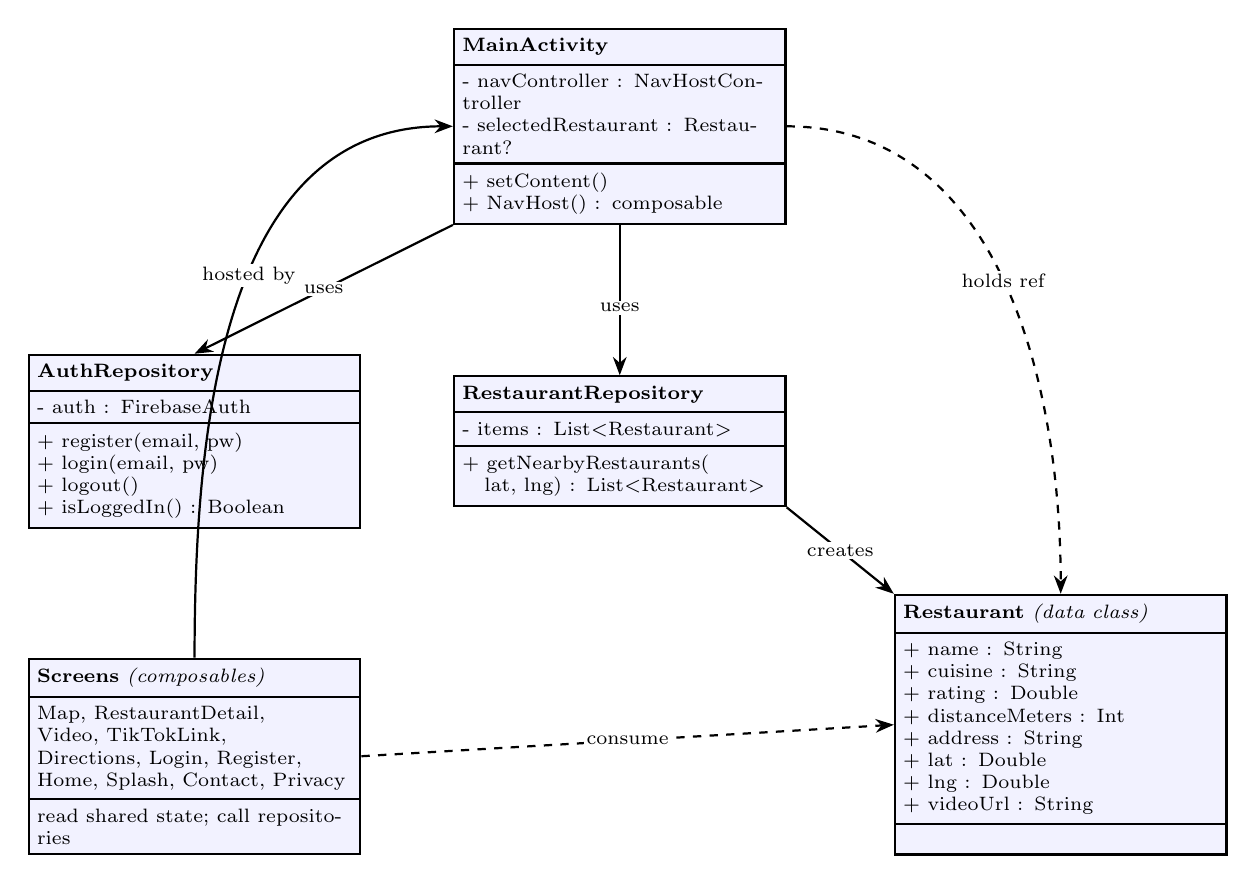
\begin{tikzpicture}[
    class/.style={
        rectangle split, rectangle split parts=3, draw, thick,
        fill=blue!5, align=left, font=\scriptsize,
        text width=4.0cm, inner sep=3pt
    },
    >=Stealth, thick
]

\node[class] (main) at (0,0) {
    \textbf{MainActivity}
    \nodepart{second}
    - navController : NavHostController\\
    - selectedRestaurant : Restaurant?
    \nodepart{third}
    + setContent()\\
    + NavHost() : composable
};

\node[class] (authrepo) at (-5.4,-4.0) {
    \textbf{AuthRepository}
    \nodepart{second}
    - auth : FirebaseAuth
    \nodepart{third}
    + register(email, pw)\\
    + login(email, pw)\\
    + logout()\\
    + isLoggedIn() : Boolean
};

\node[class] (restrepo) at (0,-4.0) {
    \textbf{RestaurantRepository}
    \nodepart{second}
    - items : List$<$Restaurant$>$
    \nodepart{third}
    + getNearbyRestaurants(\\
    \quad lat, lng) : List$<$Restaurant$>$
};

\node[class] (restaurant) at (5.6,-7.6) {
    \textbf{Restaurant} \textit{(data class)}
    \nodepart{second}
    + name : String\\
    + cuisine : String\\
    + rating : Double\\
    + distanceMeters : Int\\
    + address : String\\
    + lat : Double\\
    + lng : Double\\
    + videoUrl : String
};

\node[class] (screens) at (-5.4,-8.0) {
    \textbf{Screens} \textit{(composables)}
    \nodepart{second}
    Map, RestaurantDetail,\\
    Video, TikTokLink,\\
    Directions, Login, Register,\\
    Home, Splash, Contact, Privacy
    \nodepart{third}
    read shared state; call repositories
};

% Relationships (routed so no line crosses a class box)
\draw[->] (main.south west) -- node[font=\scriptsize, fill=white, inner sep=1pt, pos=0.5]{uses} (authrepo.north);
\draw[->] (main.south) -- node[font=\scriptsize, fill=white, inner sep=1pt, pos=0.55]{uses} (restrepo.north);
\draw[->] (restrepo.south east) -- node[font=\scriptsize, fill=white, inner sep=1pt, pos=0.5]{creates} (restaurant.north west);
% MainActivity holds a reference to the selected Restaurant (dashed, far right)
\draw[->, dashed] (main.east) to[out=0, in=90]
      node[font=\scriptsize, fill=white, inner sep=1pt, pos=0.5]{holds ref} (restaurant.north);
% Screens are hosted by MainActivity (up the left side, clear of RestaurantRepository)
\draw[->] (screens.north) to[out=90, in=180]
      node[font=\scriptsize, fill=white, inner sep=1pt, pos=0.55]{hosted by} (main.west);
% Screens consume Restaurant objects (dashed, along the bottom)
\draw[->, dashed] (screens.east) -- node[font=\scriptsize, fill=white, inner sep=1pt, pos=0.5]{consume} (restaurant.west);

\end{tikzpicture}%
}
\caption[UML class diagram of the core classes.]{UML class diagram of the core Spot To Go classes. Screens are hosted by \texttt{MainActivity} and depend on the \texttt{RestaurantRepository} interface and the \texttt{Restaurant} data type, never on the underlying data source --- the property that lets the Places API integration in Section~8 attach without changing any screen.}
\label{fig:classdiagram}
\end{figure}

\subsection{Software Architecture}

Figure~\ref{fig:arch} shows the application in four layers rather than as a sequence of screens. The point of drawing it this way is to make explicit a design decision referenced throughout this report: every screen depends only on a repository interface, never on where that repository's data actually comes from. This is why Section 8's highest-priority task — replacing the in-memory restaurant list with a live Google Places API client — is described as requiring no change to the Map screen itself; the diagram shows that dependency boundary directly.

\begin{figure}[H]
\centering
\resizebox{\textwidth}{!}{%
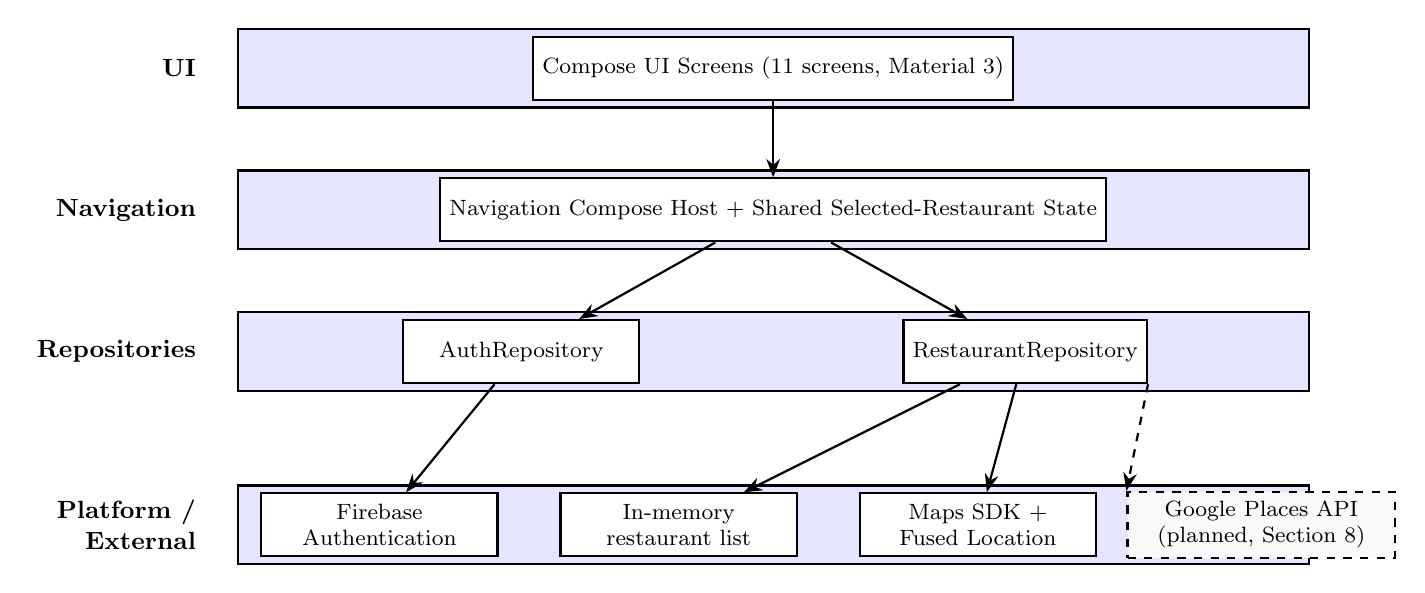
\begin{tikzpicture}[
    layer/.style={
        rectangle, draw, thick, fill=blue!10,
        minimum width=13.6cm, minimum height=1cm,
        align=center, font=\small\bfseries
    },
    box/.style={
        rectangle, draw, thick, fill=white,
        minimum width=3cm, minimum height=0.8cm,
        align=center, font=\footnotesize
    },
    future/.style={
        rectangle, draw, thick, dashed, fill=gray!5,
        minimum width=3.4cm, minimum height=0.8cm,
        align=center, font=\footnotesize
    },
    >=Stealth, thick
]

\node[layer] (uiL) at (0, 6) {};
\node[font=\small\bfseries, anchor=east] at (-7.2, 6) {UI};
\node[box] (screens) at (0, 6) {Compose UI Screens (11 screens, Material 3)};

\node[layer] (navL) at (0, 4.2) {};
\node[font=\small\bfseries, anchor=east] at (-7.2, 4.2) {Navigation};
\node[box, minimum width=8cm] (nav) at (0, 4.2) {Navigation Compose Host + Shared Selected-Restaurant State};

\node[layer] (repoL) at (0, 2.4) {};
\node[font=\small\bfseries, anchor=east] at (-7.2, 2.4) {Repositories};
\node[box] (authrepo) at (-3.2, 2.4) {AuthRepository};
\node[box] (restrepo) at (3.2, 2.4) {RestaurantRepository};

\node[layer] (svcL) at (0, 0.2) {};
\node[font=\small\bfseries, anchor=east, align=right] at (-7.2, 0.2) {Platform /\\External};
\node[box] (firebase) at (-5.0, 0.2) {Firebase\\Authentication};
\node[box] (inmem) at (-1.2, 0.2) {In-memory\\restaurant list};
\node[box] (maps) at (2.6, 0.2) {Maps SDK +\\Fused Location};
\node[future] (places) at (6.2, 0.2) {Google Places API\\(planned, Section 8)};

\draw[->] (screens) -- (nav);
\draw[->] (nav) -- (authrepo);
\draw[->] (nav) -- (restrepo);
\draw[->] (authrepo) -- (firebase);
\draw[->] (restrepo) -- (inmem);
\draw[->] (restrepo) -- (maps);
\draw[->, dashed] (restrepo.south east) -- (places.north west);

\end{tikzpicture}%
}
\caption[Layered software architecture of Spot To Go.]{Layered software architecture of Spot To Go. Screens depend only on the repository interfaces in the layer below; \texttt{RestaurantRepository} currently returns an in-memory list, and the dashed box shows where the planned Google Places API client will attach without requiring any change above the repository layer.}
\label{fig:arch}
\end{figure}

\subsection{Data Flow}

Figure~\ref{fig:dfd} shows the data flow through the application as it is currently implemented. A user first authenticates through Firebase; once signed in, the Home screen leads to the Map, which currently reads from an in-memory restaurant list rather than a live query — this stand-in is discussed further in Section 5.3 and Section 8. Selecting a marker opens the Restaurant Detail screen, from which the user can either watch a video or request directions; both actions hand off to an external app through an Android \texttt{Intent} rather than being handled inside Spot To Go itself.

\begin{figure}[H]
\centering
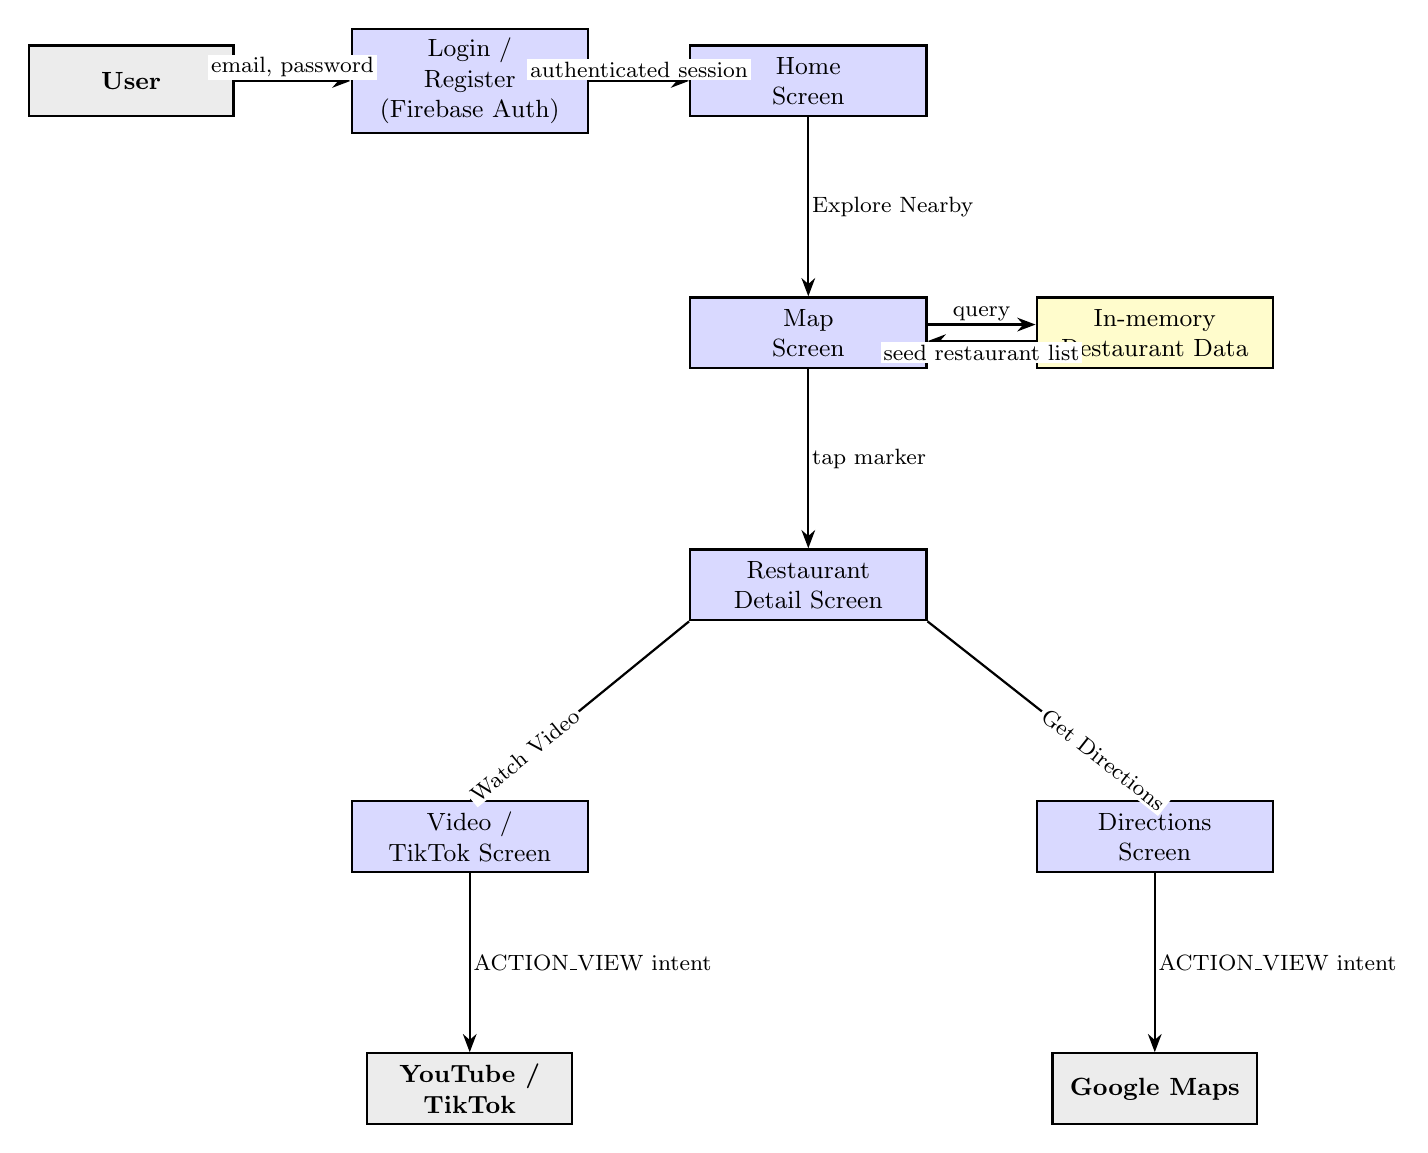
\begin{tikzpicture}[
    entity/.style={
        rectangle, draw, thick, fill=gray!15,
        minimum width=2.6cm, minimum height=0.9cm,
        align=center, font=\small\bfseries
    },
    process/.style={
        rectangle, draw, thick, fill=blue!15,
        minimum width=3cm, minimum height=0.9cm,
        align=center, font=\small
    },
    store/.style={
        rectangle, draw, thick, fill=yellow!20,
        minimum width=3cm, minimum height=0.9cm,
        align=center, font=\small
    },
    >=Stealth, thick,
    lbl/.style={font=\footnotesize, fill=white, inner sep=1pt}
]

\node[entity]  (user)   at (0,    0)    {User};
\node[process] (auth)   at (4.3,  0)    {Login /\\Register\\(Firebase Auth)};
\node[process] (home)   at (8.6,  0)    {Home\\Screen};
\node[process] (map)    at (8.6, -3.2)  {Map\\Screen};
\node[store]   (repo)   at (13,  -3.2)  {In-memory\\Restaurant Data};
\node[process] (detail) at (8.6, -6.4)  {Restaurant\\Detail Screen};
\node[process] (video)  at (4.3, -9.6)  {Video /\\TikTok Screen};
\node[process] (dir)    at (13,  -9.6)  {Directions\\Screen};
\node[entity]  (platform) at (4.3, -12.8) {YouTube /\\TikTok};
\node[entity]  (gmaps)  at (13,  -12.8) {Google Maps};

\draw[->] (user.east)   -- node[lbl, above]{email, password} (auth.west);
\draw[->] (auth.east)   -- node[lbl, above]{authenticated session} (home.west);
\draw[->] (home.south)  -- node[lbl, right]{Explore Nearby}  (map.north);
\draw[->] ([yshift= 3pt]map.east)  -- node[lbl, above]{query} ([yshift= 3pt]repo.west);
\draw[->] ([yshift=-3pt]repo.west) -- node[lbl, below]{seed restaurant list} ([yshift=-3pt]map.east);
\draw[->] (map.south)   -- node[lbl, right]{tap marker}    (detail.north);
\draw[->] (detail.south west) -- node[lbl, left, sloped]{Watch Video}     (video.north);
\draw[->] (detail.south east) -- node[lbl, right, sloped]{Get Directions} (dir.north);
\draw[->] (video.south) -- node[lbl, right]{ACTION\_VIEW intent} (platform.north);
\draw[->] (dir.south)   -- node[lbl, right]{ACTION\_VIEW intent} (gmaps.north);

\end{tikzpicture}
\caption[Data flow through the current implementation.]{Current data flow through Spot To Go. The in-memory restaurant store is a temporary stand-in for the planned Google Places API integration described in Section 8.}
\label{fig:dfd}
\end{figure}

\subsection{Application Flowchart}

Where the data flow diagram in Figure~\ref{fig:dfd} shows \emph{what} data moves between components, Figure~\ref{fig:flowchart} shows the \emph{control flow} a user actually passes through at runtime, drawn in standard flowchart notation. Rounded terminators mark the start and the two exit points, rectangles denote processing steps, and diamonds denote decisions the app makes. Presenting the flow this way makes the conditional logic explicit --- in particular the two gates that shape the experience: whether a valid session exists (which decides whether the user reaches Home or is sent to log in) and whether location permission has been granted (which decides whether the map can centre on the user's real position). The three optional branches out of the detail screen --- watch a video, get directions, or go back --- are also shown as an explicit decision rather than an implied one.

\begin{figure}[H]
\centering
\resizebox{0.82\textwidth}{!}{%
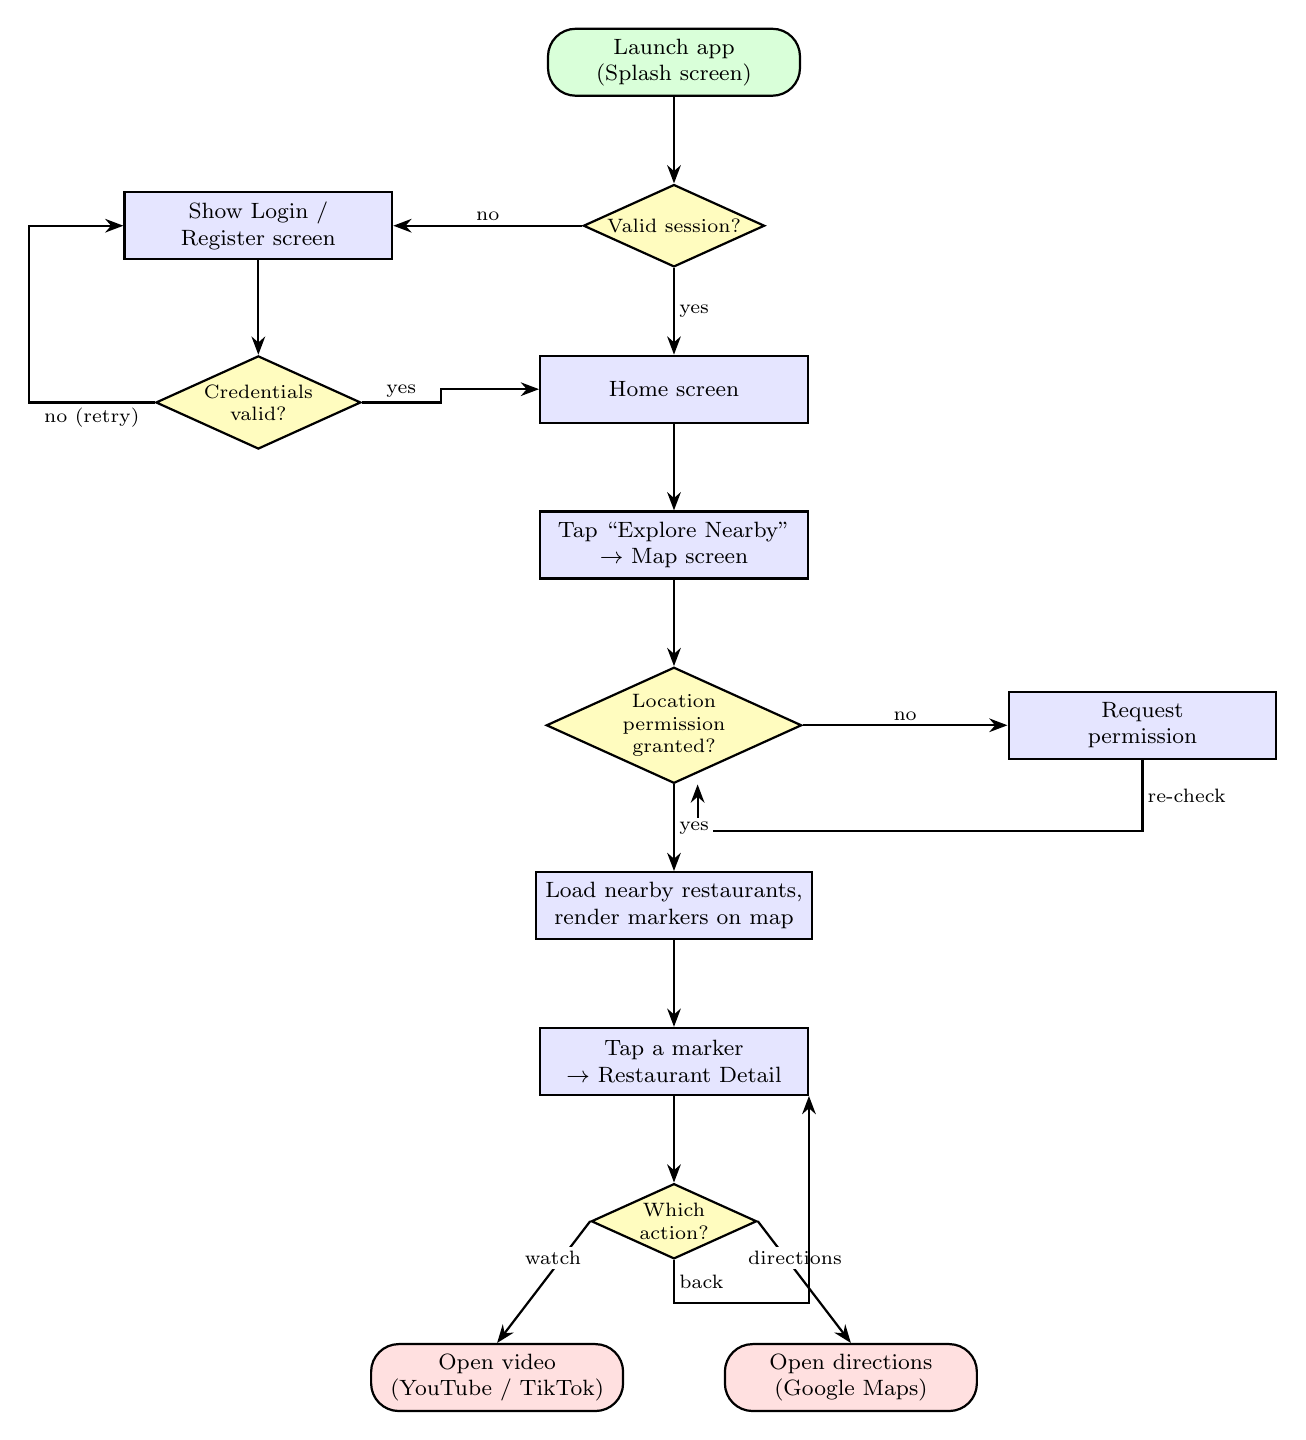
\begin{tikzpicture}[
    node distance=1.1cm and 1.6cm,
    start/.style={
        rectangle, rounded corners=10pt, draw, thick, fill=green!15,
        minimum width=3.2cm, minimum height=0.85cm, align=center, font=\footnotesize
    },
    stop/.style={
        rectangle, rounded corners=10pt, draw, thick, fill=red!12,
        minimum width=3.2cm, minimum height=0.85cm, align=center, font=\footnotesize
    },
    proc/.style={
        rectangle, draw, thick, fill=blue!10,
        minimum width=3.4cm, minimum height=0.85cm, align=center, font=\footnotesize
    },
    dec/.style={
        diamond, draw, thick, fill=yellow!25, aspect=2.2,
        inner sep=1pt, align=center, font=\scriptsize
    },
    >=Stealth, thick,
    lbl/.style={font=\scriptsize, fill=white, inner sep=1.5pt}
]

\node[start] (start) {Launch app\\(Splash screen)};
\node[dec, below=of start] (logged) {Valid session?};
\node[proc, left=2.4cm of logged] (login) {Show Login /\\Register screen};
\node[dec, below=1.2cm of login] (creds) {Credentials\\valid?};
\node[proc, below=of logged] (home) {Home screen};
\node[proc, below=of home] (explore) {Tap ``Explore Nearby''\\$\rightarrow$ Map screen};
\node[dec, below=of explore] (perm) {Location\\permission\\granted?};
\node[proc, right=2.6cm of perm] (askperm) {Request\\permission};
\node[proc, below=of perm] (loadmap) {Load nearby restaurants,\\render markers on map};
\node[proc, below=of loadmap] (tap) {Tap a marker\\$\rightarrow$ Restaurant Detail};
\node[dec, below=of tap] (action) {Which\\action?};
\node[stop, below left=1.3cm and 0.1cm of action] (video) {Open video\\(YouTube / TikTok)};
\node[stop, below right=1.3cm and 0.1cm of action] (dirs) {Open directions\\(Google Maps)};

% Main flow
\draw[->] (start) -- (logged);
\draw[->] (logged) -- node[lbl, right]{yes} (home);
\draw[->] (logged) -- node[lbl, above]{no} (login);
\draw[->] (login) -- (creds);
\draw[->] (creds.west) -- ++(-1.6,0) node[lbl, midway, below]{no (retry)} |- (login.west);
\draw[->] (creds.east) -- node[lbl, above]{yes} ++(1.0,0) |- (home.west);
\draw[->] (home) -- (explore);
\draw[->] (explore) -- (perm);
\draw[->] (perm) -- node[lbl, above]{no} (askperm);
\draw[->] (askperm.south) -- ++(0,-0.9) node[lbl, midway, right]{re-check} -| ($(perm.south)+(0.3,0)$);
\draw[->] (perm) -- node[lbl, right]{yes} (loadmap);
\draw[->] (loadmap) -- (tap);
\draw[->] (tap) -- (action);
\draw[->] (action.west) -- node[lbl, above, pos=0.4]{watch} (video.north);
\draw[->] (action.east) -- node[lbl, above, pos=0.4]{directions} (dirs.north);
\draw[->] (action.south) -- node[lbl, right]{back} ++(0,-0.55) -| (tap.south east);

\end{tikzpicture}%
}
\caption[Application flowchart of the runtime control flow.]{Application flowchart showing the runtime control flow of Spot To Go in standard notation: rounded terminators for entry and exit points, rectangles for processing steps, and diamonds for decisions. The two decision points --- session validity and location permission --- are the conditions that determine which path a user takes through the app.}
\label{fig:flowchart}
\end{figure}

% ============================================================
\section{Implementation}

\subsection{Screens}

Figure~\ref{fig:screens} shows all eleven implemented screens. Every screen is built as a Jetpack Compose function using Material 3 components, styled with a single Deep Orange (\texttt{\#FF5722}) theme applied consistently across the app.

\begin{figure}[H]
\centering
\shot{0.15\textwidth}{splash screen.jpeg}{Splash screen shown briefly on launch while the app loads and checks for a session.}
\hfill\shot{0.15\textwidth}{home page.jpeg}{Home screen with the keyword search bar and the Explore Nearby button leading to the map.}
\hfill\shot{0.15\textwidth}{login page.jpeg}{Login screen where an existing user signs in with email and password through Firebase Authentication.}
\hfill\shot{0.15\textwidth}{registration page.jpeg}{Registration screen creating a new Firebase account from an email, password, and display name.}
\hfill\shot{0.15\textwidth}{map page.jpeg}{Map centred on the user's real GPS location, showing nearby restaurants as tappable markers.}
\hfill\shot{0.15\textwidth}{hotel review page.jpeg}{Restaurant detail screen showing name, rating, distance, address, and description with action buttons.}

\vspace{4mm}

\shot{0.18\textwidth}{watch video page.jpeg}{Video screen that opens a real YouTube preview of the restaurant through an Android intent.}
\hfill\shot{0.18\textwidth}{tiktok launch page.jpeg}{TikTok link screen, styled like a post, opening a TikTok search for the restaurant.}
\hfill\shot{0.18\textwidth}{direction screen.jpeg}{Directions screen offering car, bus, and walk modes before launching Google Maps navigation.}
\hfill\shot{0.18\textwidth}{contact us page.jpeg}{Contact Us screen giving users a simple channel to reach the developers of the app.}
\hfill\shot{0.18\textwidth}{privacy page.jpeg}{Privacy Policy screen summarising how location data and account details are used and stored.}
\caption[The eleven implemented screens.]{All eleven implemented screens, matching the flow shown in Figure~\ref{fig:prototype}.}
\label{fig:screens}
\end{figure}

\subsection{Location and Mapping}

The Map screen uses the Fused Location Provider (\texttt{FusedLocationProviderClient}), Google's recommended location API on Android \citep{android_location}, to read the device's last known location, after requesting the \texttt{ACCESS\_FINE\_LOCATION} runtime permission through the Accompanist Permissions library. The map itself is rendered with the Maps Compose library (\texttt{com.google.maps.android.compose}), which wraps the native Google Maps SDK for use inside a composable. Each restaurant is shown as a marker with the restaurant's name and a snippet combining its cuisine and rating; tapping a marker opens the Restaurant Detail screen for that restaurant. The Directions screen uses the same pattern independently, so that if the user's location changes between viewing the map and requesting directions, the directions screen still reflects a current position.

\subsection{Restaurant Data}

Restaurant data is currently served by \texttt{RestaurantRepository}, which returns a fixed, in-memory list of five restaurants (spanning Indian, Chinese, Italian, American, and Japanese cuisine) positioned at small fixed offsets from the user's real coordinates, so that markers appear plausibly ``nearby'' regardless of where the app is run. Each restaurant record carries a name, cuisine, rating, computed distance, address, coordinates, and a real YouTube video URL. This repository was deliberately built behind a single interface consumed by the Map screen, so that replacing it with a live Google Places API client — the next piece of work, described in Section 8 — requires no change to the Map screen itself.

\subsection{Video and Directions}

Rather than embedding video playback inside the app with a \texttt{WebView}, the Video screen dispatches the restaurant's YouTube URL through an Android \texttt{Intent} with action \texttt{ACTION\_VIEW}, which the operating system hands to the installed YouTube app or, failing that, a browser. A second button on the same screen leads to a TikTok Link screen, styled to resemble a TikTok post, which in turn opens a TikTok search for the restaurant's name through the same \texttt{ACTION\_VIEW} mechanism. Directions follow an equivalent pattern: the Directions screen builds a Google Maps web URL from the user's current coordinates and the restaurant's coordinates, with the selected transport mode (car, bus, or walk) encoded in the URL, and dispatches it through \texttt{ACTION\_VIEW} so that the installed Google Maps app opens with turn-by-turn directions already configured.

\subsection{Authentication}

Login and registration are backed by Firebase Authentication \citep{firebase_auth} through a single \texttt{AuthRepository} object, exposing \texttt{register}, \texttt{login}, \texttt{logout}, and an \texttt{isLoggedIn} check. Registration creates a Firebase user with email and password and sets the user's display name; login signs an existing user in through the same mechanism. The Map screen checks \texttt{isLoggedIn} itself and redirects to the Login screen if no session is active, so that the map — and everything reachable from it — is gated behind a real sign-in rather than a hardcoded credential check as originally proposed. This has been tested end-to-end on a physical Android device: registering a new account, being signed in automatically, and reaching the map.

Figure~\ref{fig:authseq} sets out that tested flow as a sequence diagram, showing which calls are handled inside the app and which are delegated to Firebase.

\begin{figure}[H]
\centering
\resizebox{\textwidth}{!}{%
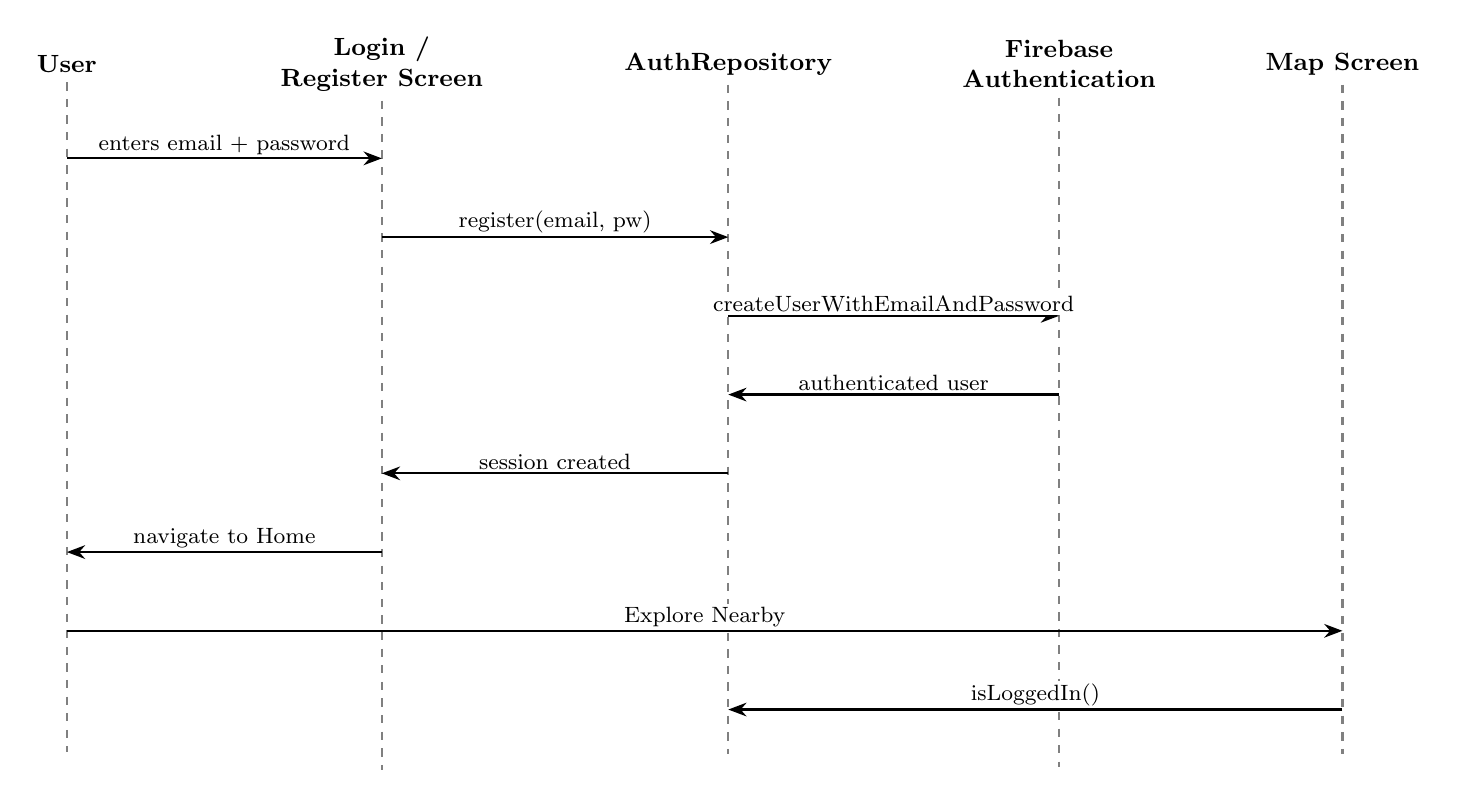
\begin{tikzpicture}[
    actor/.style={font=\small\bfseries, align=center},
    lifeline/.style={dashed, thick, gray},
    msg/.style={->, thick, >=Stealth},
    lbl/.style={font=\footnotesize, fill=white, inner sep=1pt}
]

\def\yTop{0}
\def\yBot{-8.5}

\node[actor] (user) at (0, \yTop) {User};
\node[actor] (screen) at (4, \yTop) {Login /\\Register Screen};
\node[actor] (repo) at (8.4, \yTop) {AuthRepository};
\node[actor] (firebase) at (12.6, \yTop) {Firebase\\Authentication};
\node[actor] (map) at (16.2, \yTop) {Map Screen};

\draw[lifeline] (user.south)     -- ++(0, \yBot);
\draw[lifeline] (screen.south)   -- ++(0, \yBot);
\draw[lifeline] (repo.south)     -- ++(0, \yBot);
\draw[lifeline] (firebase.south) -- ++(0, \yBot);
\draw[lifeline] (map.south)      -- ++(0, \yBot);

\draw[msg] (0,-1.2)   -- node[lbl, above]{enters email + password} (4,-1.2);
\draw[msg] (4,-2.2)   -- node[lbl, above]{register(email, pw)} (8.4,-2.2);
\draw[msg] (8.4,-3.2) -- node[lbl, above]{createUserWithEmailAndPassword} (12.6,-3.2);
\draw[msg] (12.6,-4.2) -- node[lbl, above]{authenticated user} (8.4,-4.2);
\draw[msg] (8.4,-5.2) -- node[lbl, above]{session created} (4,-5.2);
\draw[msg] (4,-6.2)  -- node[lbl, above]{navigate to Home} (0,-6.2);
\draw[msg] (0,-7.2)  -- node[lbl, above]{Explore Nearby} (16.2,-7.2);
\draw[msg] (16.2,-8.2) -- node[lbl, above]{isLoggedIn()} (8.4,-8.2);

\end{tikzpicture}%
}
\caption[Sequence diagram of the authentication flow.]{Sequence diagram of the tested authentication flow, from account registration through to the Map screen's own session check. \texttt{AuthRepository} is the only component that talks to Firebase directly; the Map screen re-checks \texttt{isLoggedIn} independently so it can never be reached without a valid session, regardless of how it was navigated to.}
\label{fig:authseq}
\end{figure}

\subsection{Navigation and State}

All eleven screens are connected through a single Navigation Compose host defined in \texttt{MainActivity}, with the splash screen as the start destination. Rather than passing the selected restaurant as a navigation argument on every route, the app holds it as a single piece of shared Compose state at the navigation level, set whenever a restaurant is chosen from the map. The Detail, Video, TikTok, and Directions screens all read from this same value, so the currently selected restaurant survives navigating between them.

\subsection{Deviations from the Original Proposal}

Four implementation choices depart from the proposal, summarised here for transparency:

\begin{itemize}
    \item \textbf{Kotlin and Jetpack Compose instead of Java and Activities.} Justified above in Section 4.1; permitted by the project brief and better suited to sharing state between screens.
    \item \textbf{Real Firebase Authentication instead of hardcoded credentials.} The proposal treated login as a demonstration screen with no live backend, to avoid handling real personal data. The implemented app uses real Firebase Authentication instead, because gating the map behind a genuine sign-in makes the ``informed decision-making'' narrative of the app more credible during a live demonstration, and because Firebase Authentication is a managed service that stores credentials securely without the project needing to run its own user database. Section 7.2 revisits the ethical implications of this change.
    \item \textbf{Intent-based video playback instead of an in-app \texttt{WebView}.} Handing playback to the installed YouTube or TikTok app is simpler to implement, matches how users already expect to watch video content on their phone, and avoids the extra permissions and edge cases that come with embedding a web view.
    \item \textbf{A Google Maps web-intent URL instead of a \texttt{geo:} URI for directions.} The web-intent form still opens the native Google Maps app when it is installed, but falls back gracefully to a browser when it is not, which is a safer default for a device configuration that has not been tested in advance.
\end{itemize}

% ============================================================
\section{Testing and Evaluation}

\subsection{Functional Testing}

Testing to date has been carried out informally on a physical Android device rather than through the structured, objective-by-objective test plan proposed earlier, and this remains an open task noted in Section 8. That said, the core flow — opening the app, registering an account, being signed in automatically, viewing the map, opening a restaurant's detail screen, watching its video, and requesting directions — has been exercised directly and works as intended.

This testing surfaced five issues, all of which have since been fixed:
\begin{itemize}
    \item The on-screen keyboard was covering the password field on the Login and Registration screens; resolved by applying \texttt{imePadding} so the form scrolls clear of the keyboard.
    \item There was no way to check a password had been typed correctly before submitting; resolved by adding a show/hide toggle to both password fields.
    \item The Map screen had no way back to the rest of the app other than the phone's back button, which simply exited the app; resolved by adding a bottom navigation bar consistent with the Home screen.
    \item The Home screen's navigation bar showed a ``Login'' option even when a user was already signed in; resolved by having both navigation bars read the same \texttt{isLoggedIn} state.
    \item The Login screen's ``Continue as Guest'' option bypassed Firebase Auth entirely and, once the Map screen was gated on a signed-in session, sent guest users into a redirect loop; the button was removed. The Login screenshot in Figure~\ref{fig:screens} was captured before this fix and still shows the button, which has since been removed from the app.
\end{itemize}

\subsection{Usability Considerations}

A lightweight heuristic pass, following \citet{nielsen1994}, was applied informally during the fixes above rather than as a separate, scheduled review. Of the ten heuristics, four are most directly relevant to this app: visibility of system status, match between the system and the real world, user control and freedom, and error prevention. The user-control issue identified above (the map's earlier dead end) has been resolved; a related, smaller issue — that pressing back on the map screen still exits the app immediately, since it is the first screen reached after login — remains open and is listed as a task in Section 8. The formal second stage proposed earlier, in which three to five participants complete a defined task list and a System Usability Scale questionnaire, has not yet been run and is scheduled for after the Places API integration is complete, so that participants test against live restaurant data rather than the placeholder list.

% ============================================================
\section{Analysis of Risks and Ethical Issues}

\subsection{Technical Risks}

The Google Places API request quota risk described in the proposal has not yet materialised, since the app currently runs entirely on in-memory data and makes no calls to the Places API. This risk becomes active as soon as the integration described in Section 8 begins, and will be managed as originally planned: by caching responses where they are stable and by controlling request frequency during testing.

The risk that linked video content may be removed or become unavailable still applies to the five video URLs currently seeded into the app, and is mitigated in the same way as proposed — by choosing stable, established videos for demonstration purposes.

Device fragmentation remains a live consideration. The app currently targets a minimum SDK of API level 24 and a target SDK of API level 36, which covers the large majority of active Android devices; testing so far has been carried out on a single physical device, and testing across a wider range of screen sizes and OS versions remains outstanding.

\subsection{Ethical Considerations}

This section is the one most significantly affected by the deviation described in Section 5.7. The proposal stated that login would be demonstration-only, collecting no real personal data. The implemented app instead uses real Firebase Authentication, which does collect a genuine email address and password for any user who registers. This changes the ethical position of the project and needs to be stated plainly rather than carried over unchanged from the proposal.

In practice, the risk this introduces is small and well-managed. Firebase Authentication is a managed identity service operated by Google; passwords are never stored or handled directly by the application's own code, and no additional personal data — beyond the email address and display name required to sign in — is collected or stored anywhere in the app. No Firestore database or other persistent store of user data is used. Location data continues to be used only transiently, to centre the map and compute the placeholder restaurant positions, and is not stored beyond the current session. Because the accounts created during testing are the developer's own test accounts rather than data from human participants, and because no analytics or third-party tracking is integrated, the change does not introduce a need for formal ethical approval; it does, however, mean that any demonstration or further testing involving other people's real credentials should be limited to consenting testers who understand that a genuine account is being created.

% ============================================================
\section{Current Progress and Remaining Work}

\subsection{Project Schedule}

The work was planned against a fixed submission deadline, so the project was divided into seven sequential work packages and scheduled across the available months rather than left open-ended. Figure~\ref{fig:gantt} presents this plan as a Gantt chart, with each work package (WP1--WP7) mapped to a calendar window from April to September 2026. The packages were deliberately allowed to overlap where a later stage could begin before the previous one was fully closed --- for example, screen implementation (WP3--WP5) was staged so that mapping, detail/video, and search work could run into one another rather than waiting for a clean handover --- which kept progress continuous instead of stalling at package boundaries. As of the date of this draft, WP1 through WP5 are complete and WP6 (Testing and Writing) is in progress; the finer-grained dependency view of the tasks that remain within these final packages is given separately in Figure~\ref{fig:roadmap}.

\begin{figure}[H]
\centering
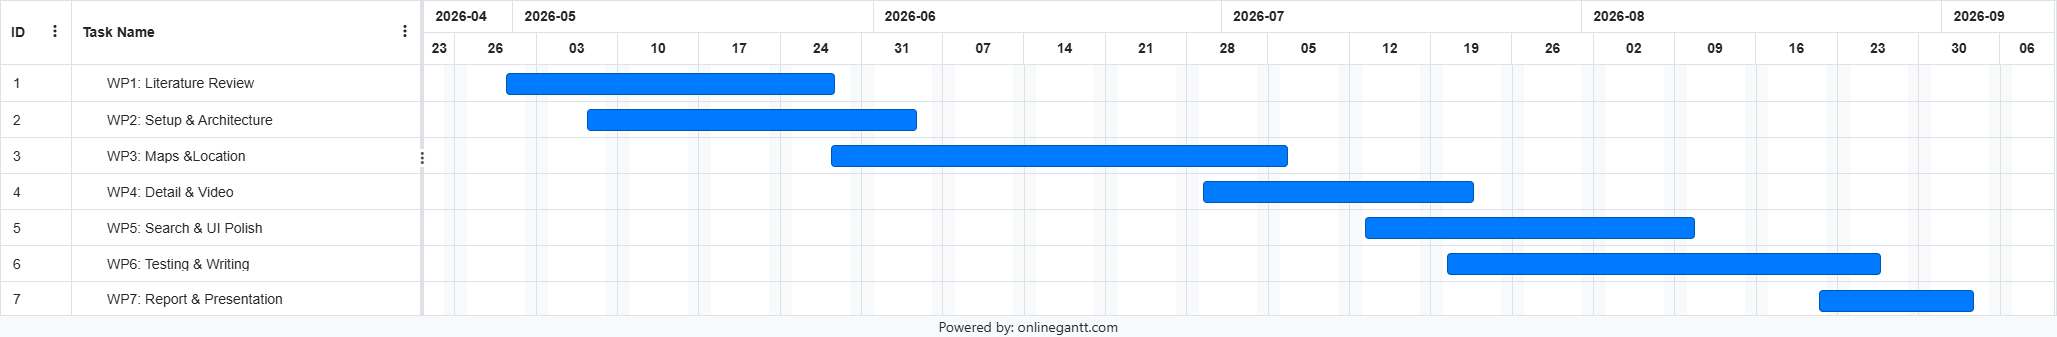
\includegraphics[width=\textwidth]{images/gant chart.png}
\caption[Project schedule Gantt chart (WP1--WP7).]{Project schedule across seven work packages (WP1--WP7), from the literature review through to final report and presentation. The chart shows the planned calendar window for each package; overlaps between adjacent packages were intentional, allowing later implementation stages to begin before the previous one was fully closed.}
\label{fig:gantt}
\end{figure}

\subsection{Summary of Progress}

All eleven planned screens are implemented and connected through a single navigation flow. The map renders live using the device's real GPS location and the Google Maps SDK. Firebase Authentication is live and has been tested end-to-end on a physical device, including the UX fixes listed in Section 6.1. Video and directions both work by handing off to external apps through Android intents, and the search bar filters the currently loaded restaurant list in real time.

\subsection{Remaining Work}

Three pieces of work are outstanding, in priority order:

\begin{enumerate}
    \item \textbf{Google Places Nearby Search API.} Replace \texttt{RestaurantRepository}'s in-memory list with a new repository backed by a live Nearby Search call \citep{google_places} (type \texttt{restaurant}, radius 1500 metres), returning real restaurants around the user's location. Because the Map screen already depends only on the repository's interface, this screen requires no changes of its own.
    \item \textbf{Live search.} Once real restaurant data is flowing, connect the existing search bar to the Places API's keyword parameter with a short debounce, replacing the current client-side filter over the placeholder list, and show a loading indicator while a search request is in flight.
    \item \textbf{Back-press polish and formal testing.} Add a press-back-again-to-exit confirmation on the Map screen, and carry out the structured functional test plan and the participant-based usability testing (Section 6.2) that were deferred until real restaurant data is available to test against.
\end{enumerate}

Figure~\ref{fig:roadmap} sets out the same three items as a dependency chain rather than a dated schedule, since no fixed dates have been committed to at this stage of the project. The ordering reflects a genuine dependency, not just a preference: live search cannot be connected to the Places API's keyword parameter (item 2) until that API call exists at all (item 1), whereas the back-press and testing work (item 3) is independent and could, in principle, proceed in parallel.

\begin{figure}[H]
\centering
\resizebox{\textwidth}{!}{%
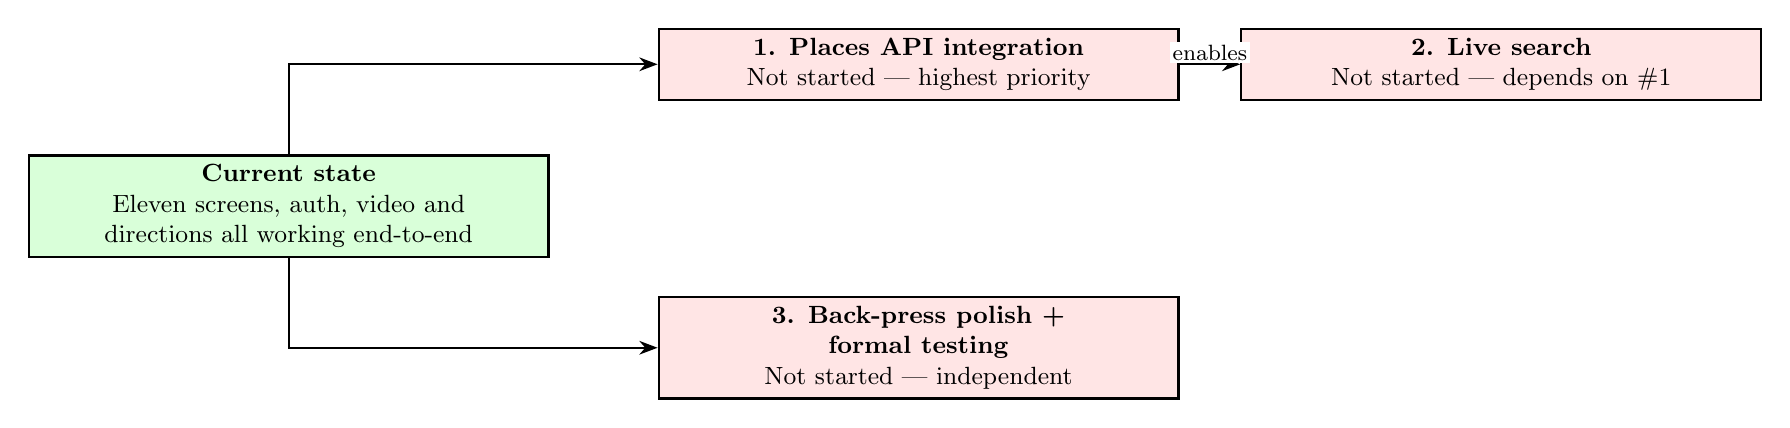
\begin{tikzpicture}[
    done/.style={
        rectangle, draw, thick, fill=green!15,
        minimum width=6.6cm, minimum height=0.9cm,
        align=center, font=\small
    },
    todo/.style={
        rectangle, draw, thick, fill=red!10,
        minimum width=6.6cm, minimum height=0.9cm,
        align=center, font=\small
    },
    >=Stealth, thick,
    lbl/.style={font=\footnotesize, fill=white, inner sep=1pt}
]

\node[done] (current) at (0, 0)     {\textbf{Current state}\\Eleven screens, auth, video and\\directions all working end-to-end};
\node[todo] (places)  at (8, 1.8)   {\textbf{1. Places API integration}\\Not started --- highest priority};
\node[todo] (search)  at (15.4, 1.8) {\textbf{2. Live search}\\Not started --- depends on \#1};
\node[todo] (testing) at (8, -1.8)  {\textbf{3. Back-press polish +}\\\textbf{formal testing}\\Not started --- independent};

\draw[->] (current.north) |- (places.west);
\draw[->] (current.south) |- (testing.west);
\draw[->] (places) -- node[lbl, above]{enables} (search);

\end{tikzpicture}%
}
\caption[Remaining work as a dependency chain.]{Remaining work as a dependency chain rather than a dated roadmap. The Places API integration (Section 8, item 1) blocks live search (item 2); formal back-press and usability testing (item 3) does not depend on either and could run in parallel.}
\label{fig:roadmap}
\end{figure}

% ============================================================
\section{Conclusion}

Spot To Go has progressed from a proposal into a working Android application. Every screen from the original prototype has been built, styled consistently, and connected into a single, tested navigation flow; a real authentication system gates access to the map; and the map itself renders the user's true location alongside restaurants that can be explored through a real video preview or turned into real driving, walking, or transit directions with a single tap. The one substantive gap against the original objectives is the live Google Places API integration, which remains the clearly scoped next step — the surrounding architecture was built specifically so that this change would not require reworking any of the screens already in place.

The purpose of this draft is to put that progress in front of a reviewer before the remaining work begins, so that feedback on the screens, the architecture, and the ethical position described in Section 7.2 can shape how the final phase of the project is prioritised.

% ============================================================
\newpage
\bibliographystyle{apalike}
\bibliography{references}

\end{document}
